Benchmark-ul cGAN aparține mulțimii de benchmark-uri din cadrul competiției VNN-COMP 2023 \cite{vnncompBenchmarks}. Acesta conține o rețea de tip generativă adversarială condiționată și un set de specificații. Benchmark-ul este folosit pentru a verifica corectitudinea și robustețea rețelei pe care o conține. În cadrul set-ului de date, există două tipuri de fișiere: .onnx (Open Neural Network Exchange) și .vnnlib. În fișierele .onnx sunt reprezentate rețele neuronale, acestea conțin informații necesare pentru a executa modelul neuronal. Fișierele .vnnlib conțin specificațiile ce trebuie respectate de rețeaua neuronală, astfel încât aceasta să fie corectă și robustă.

Atât fișierele .onnx cât și .vnnlib au o denumire sugestivă care să indice informații despre conținutul acestora.
\begin{figure}[ht]
\begin{tabular}{cc}
\hspace{-2cm} \subfloat[Fișiere .onnx]{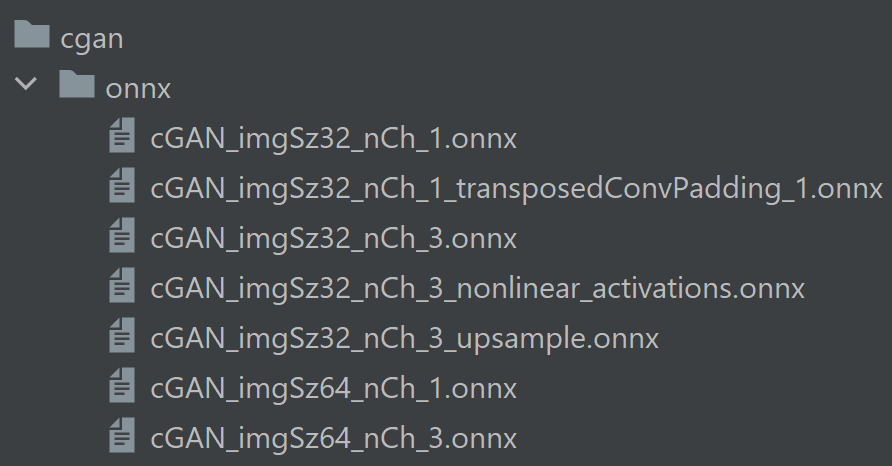
\includegraphics[width=7.5cm]{imagini/caracterizareSetDate/onnx.png}} &
\hspace{-0.5cm} \subfloat[Fișiere .vnnlib]{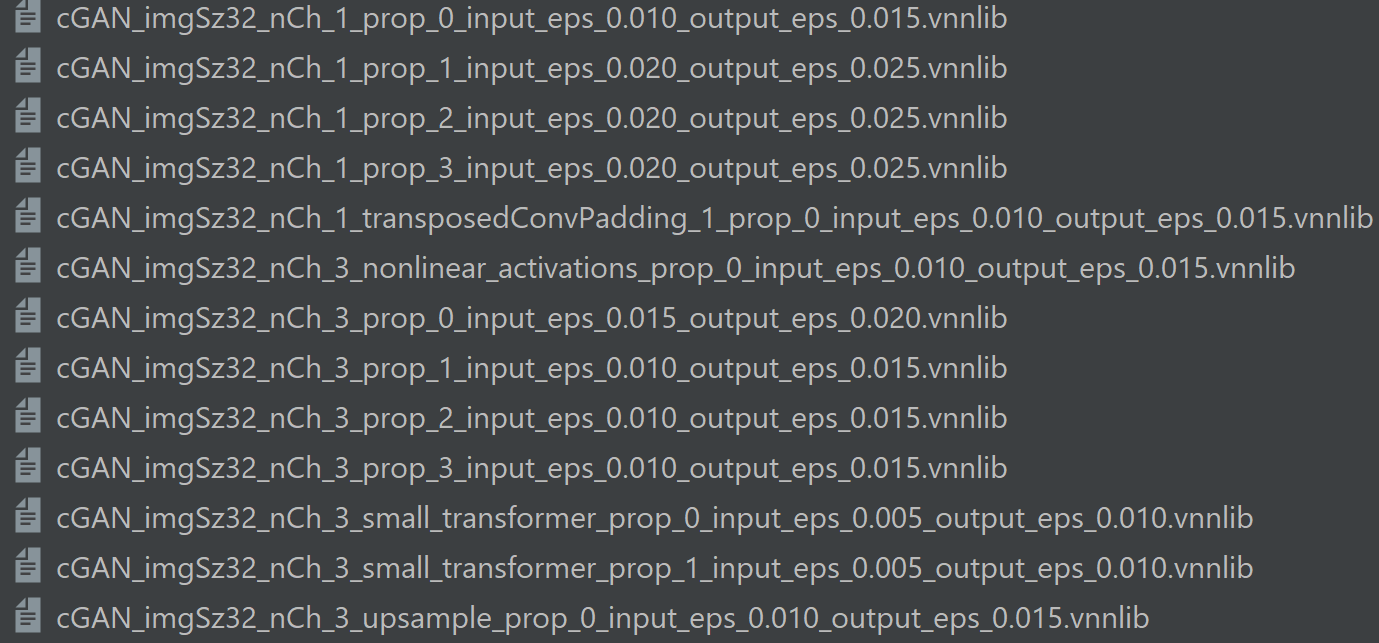
\includegraphics[width=10cm]{imagini/caracterizareSetDate/vnnlib.png}}
\end{tabular}
\caption{Fișierele benchmark-ului cGAN}
\end{figure}
\begin{itemize}
  \item \textit{CGan} - tipul de rețea neurală, în acest caz, o rețea generatoare adversarială condiționată.
  
  \item \textit{imgSz32} - dimensiunea imaginei generate, în acest caz, o dimensiune de 32x32 pixeli.

  \item \textit{nCh\_1} - numărul de canale de culoare utilizate în imaginile de intrare sau de ieșire ale rețelei.
  
  \item \textit{prop\_0} - parametru/proprietate specifică a imaginei

  \item \textit{input\_eps\_0} - valoare epsilon utilizată peste datele de intrare ale rețelei.
  
  \item \textit{output\_eps\_0.015} -  valoare epsilon utilizată peste datle de ieșire a rețelei.


  \item \textit{transportedConvPadding\_1} - tip specific de convoluție a rețelei.
  
  \item \textit{nonlinear\_activations} - rețeaua conține funcții de activare non-liniare între straturi.

  \item \textit{upsample} - modelul neuronal efectuează operații de upsampling, care sunt utilizate pentru a mări dimensiunea spațială a imaginilor sau a datelor. Aceasta poate fi utilă în cazul modelelor generatoare pentru a genera imagini de rezoluție mai mare sau în alte scenarii în care este necesară mărirea dimensiunii datelor.
  
\end{itemize}